\documentclass{beamer}
\usepackage[utf8]{inputenc}

%Information to be included in the title page:
\title{Seminar Talk \\ F09: Neuromorphic Computing}
\author{Students: Robin Dorstijn \& Moritz Epping \\ Supervisor: Jakob Kaiser}
\institute{Universität Heidelberg}
\date{January 2021}

\usepackage{import}
\usepackage{xifthen}
\usepackage{pdfpages}
\usepackage{transparent}
\usepackage{titlesec}


\newcommand{\incfig}[1]{
    \def\svgwidth{\columnwidth}
    \import{./figures/}{#1.pdf_tex}
}

\begin{document}

\frame{\titlepage}

\begin{frame}
    %%%
    \frametitle{Summary}
    \begin{enumerate}
        \item Theoretical Overview
        \item Results
        \item Discussion
    \end{enumerate}
    %%%
\end{frame}

\begin{frame}
    %%%
    \frametitle{Motivation}
   	\begin{itemize}
   		\item Goals of Neuromorphic Computing:
   		\begin{enumerate}
   			\item Building more efficient computers (Von-Neumann Bottleneck vs.  Evolution)
   			\item  Understanding brain by trying to rebuild it!
   		\end{enumerate}
   		\bigskip
   		\item Proposed Architecture: SPIKEY (Heidelberg)
   		\begin{enumerate}
   			\item What are basic properties neuromorphic computing devices must fulfill?
   			\item Does SPIKEY fulfill these properties?
   			\item How well can we use it for more complicated purposes?
   		\end{enumerate}
   	\end{itemize}
\end{frame}

\begin{frame}
    %%%
    \frametitle{Theoretical Overview - Neurons}
    \begin{columns}
          \column{0.28\linewidth}
             \centering
             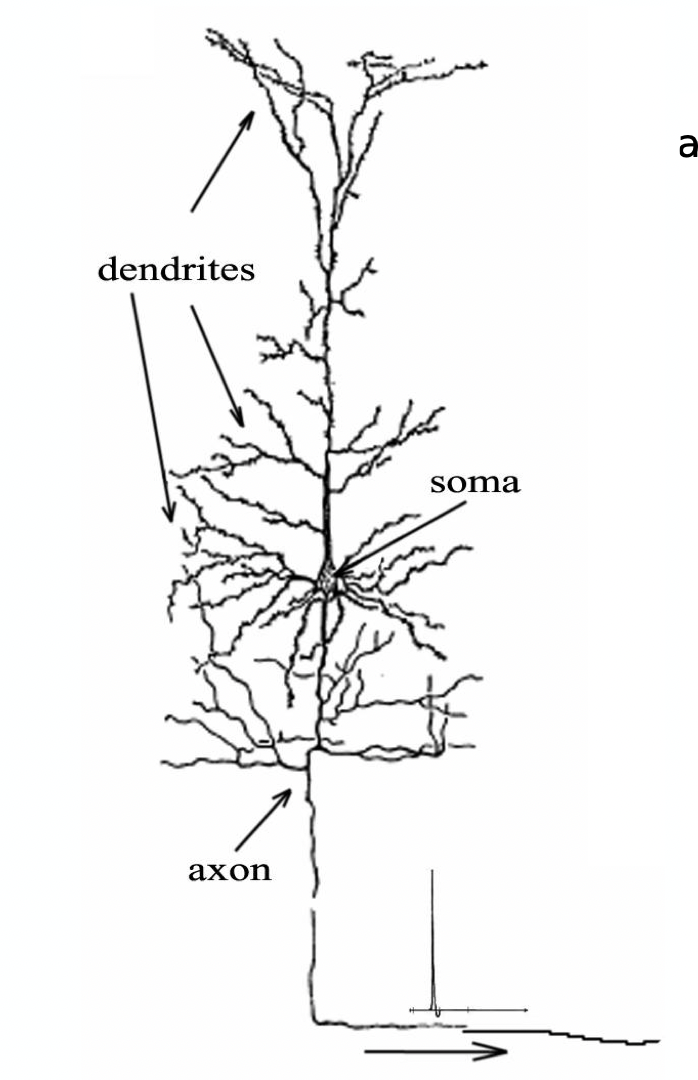
\includegraphics[height=5cm, width=3.5cm]{figures/neuron_script.png}
           \column{0.68\linewidth}
              \begin{itemize}

   				\item Biological Neuron
   				\begin{itemize}
   					\item Basic computational units of the brain
   					\item Electronic information processing
   					\item Receive input signals (ion waves) via \textbf{dendrites}
   					\item Depending on input: Create a signal
   					\item Transmit signal to other neurons
   				\end{itemize}

   				\item form a network with several interconnected neurons
 			\end{itemize}
	\end{columns}

\end{frame}

\begin{frame}
    %%%

    \frametitle{Theoretical Overview - LiF Model}

     \begin{figure}
    		\centering
    		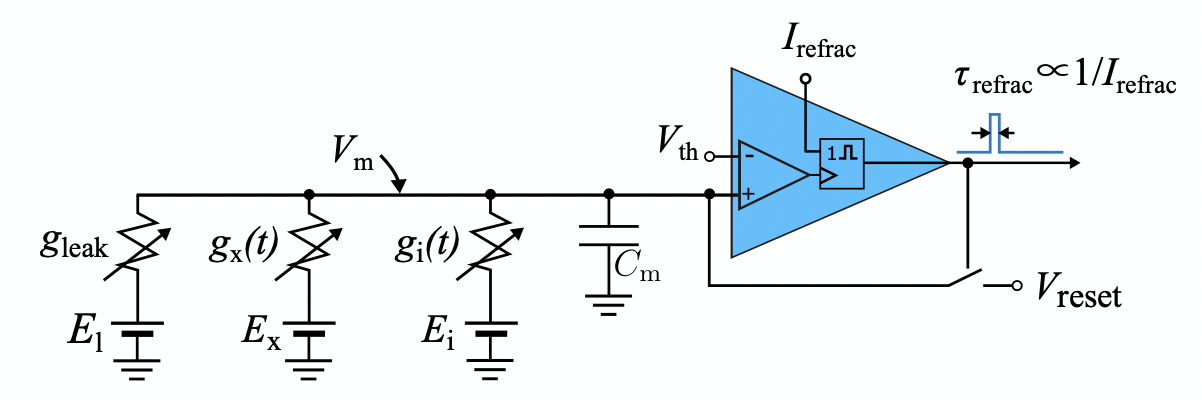
\includegraphics[width=0.8\textwidth]{figures/lif_script.png}
    		%\caption{source: FP09 neuromorphic computing script,  2020}
    \end{figure}

     \begin{itemize}

   		\item Electronical Analogy: LIF - Circuit
   		\begin{itemize}
   				\item \textbf{L}eaky \textbf{I}ntegrate and \textbf{F}ire
   				\item Treat neuron as capacitor
   				\item Currents charging / decharging it (input)
   				\item Op-Amp: Compare capacitor voltage to \textit{threshold voltage},  if
   				$V\geq V_{th}$ then spike
   		\end{itemize}
 	\end{itemize}

\end{frame}

\begin{frame}
	\frametitle{Hardware realization: Spikey}
	\begin{columns}
          \column{0.5\linewidth}
          	\begin{figure}
    				\centering
    				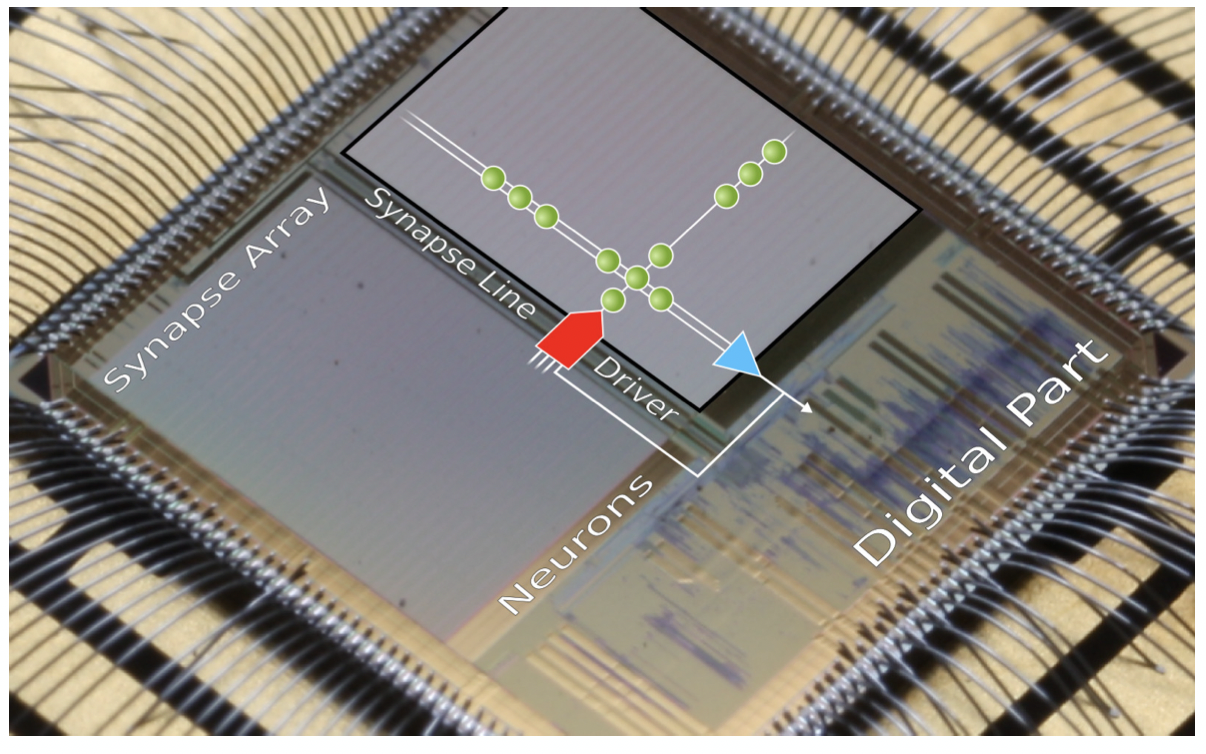
\includegraphics[width=\linewidth]{figures/script_spikey_image.png}
    				%\caption{source: FP09 neuromorphic computing script,  2020}
 		   \end{figure}
 		   \begin{itemize}
          		\item Spikey as a collection of LiF circuits interconnected with synapses
          	\end{itemize}

          \column{0.5\linewidth}
          \begin{figure}
    				\centering
    				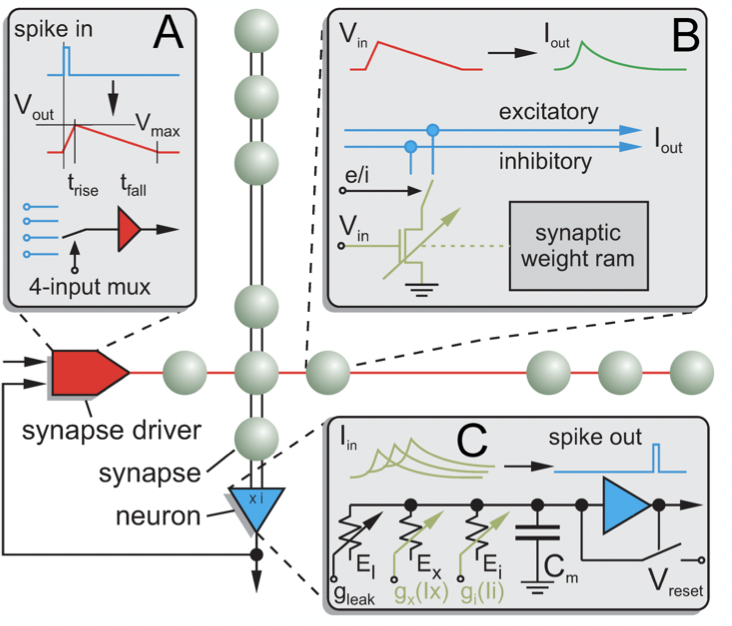
\includegraphics[width=\linewidth]{figures/script_spikey_schematic.png}
    				%\caption{source: FP09 neuromorphic computing script,  2020}
 		   \end{figure}
 		   \begin{itemize}
          		\item Schematic of the basic operation process
          	\end{itemize}

	\end{columns}
\end{frame}


\begin{frame}
    %%%
    \frametitle{Results - 1: basic firing behaviour}
    %%%
    \begin{figure}
    		\centering
    		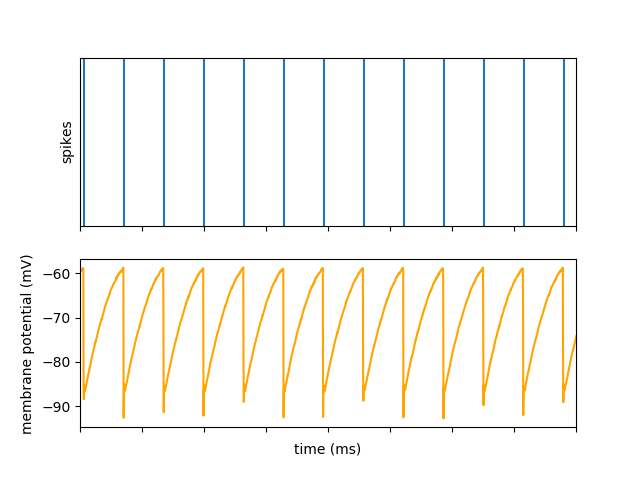
\includegraphics[width=0.6\linewidth]{figures/fp_task1_1membrane.png}
    \end{figure}

    \begin{itemize}
    		\item no excitatory/inhibitory synapses,  just leakage potential,
    		\textbf{but: } $E_l>V_{th}\quad \Rightarrow$ Spikes
    		\item Firing rate measured to $t_{fir} = (16.10\pm 0.11)$; dependent on
    		time constant, leakage potential,  leakage conductance
    \end{itemize}
\end{frame}

\begin{frame}
    %%%
    \frametitle{Results - 1: basic firing behaviour}
    %%%
\end{frame}

\begin{frame}
    %%%M
    \frametitle{Results - 1: single neuron}
    %%%


\end{frame}

\begin{frame}
    %%%R
    \frametitle{Results - 2: calibrating neuron parameters}
    %%%
    \begin{figure}
        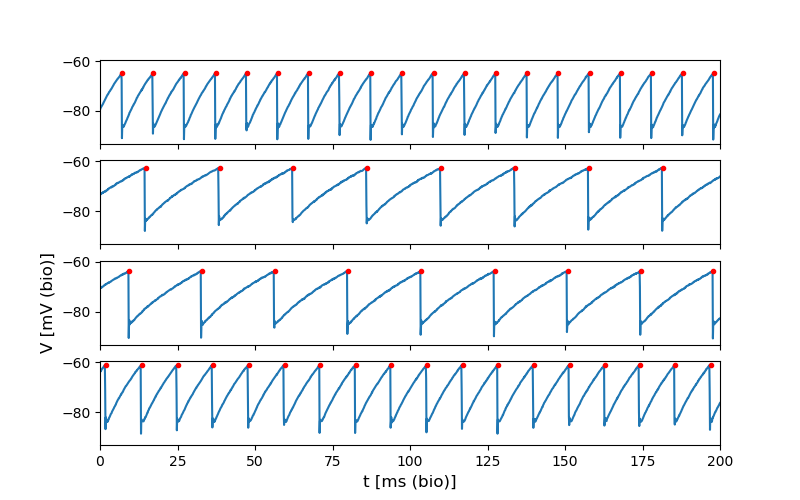
\includegraphics[width=.7\textwidth]{figures/4membranes.png}
        \caption{4 uncalibrated neurons firing at natural time constants.}
    \end{figure}
    \begin{itemize}
        \item Uncalibrated neurons differ in time constants
        \item Calibration required before effective running
    \end{itemize}
\end{frame}

\begin{frame}
    %%%R
    \frametitle{Results - 2: calibrating neuron parameters}
    Suggested algorithm:
    \begin{enumerate}
        \item Set the $g_l$ to the default value and measure the rate of the neuron.
        \item Set the $g_l$ to double the default value and measure the rate of the
            neuron.
        \item Describe the response of the neuron linearly using the last two
            points and estimate where the desired rate would lie.
        \item Set the $g_l$ to this value and measure the rate, if it is within the
        standard error: success! If not return to step 3.
    \end{enumerate}
\end{frame}

\begin{frame}
    %%%R
    \frametitle{Results - 2: calibrating neuron parameters}
    \begin{figure}
        \incfig{algo-base}
    \end{figure}
\end{frame}

\begin{frame}
    %%%R
    \frametitle{Results - 2: calibrating neuron parameters}
    \begin{figure}
        \incfig{algo-1,2}
    \end{figure}
\end{frame}

\begin{frame}
    %%%R
    \frametitle{Results - 2: calibrating neuron parameters}
    \begin{figure}
        \incfig{algo-3}
    \end{figure}
\end{frame}

\begin{frame}
    %%%R
    \frametitle{Results - 2: calibrating neuron parameters}
    \begin{figure}
        \incfig{algo-4}
    \end{figure}
\end{frame}

\begin{frame}
    %%%R
    \frametitle{Results - 2: calibrating neuron parameters}
    \begin{figure}
        \incfig{algo-3-repeat}
    \end{figure}
\end{frame}

\begin{frame}
    %%%M
    \frametitle{Results - 3: single neuron with synaptic input}
    %%%
    \begin{itemize}
    		\item we need to evaluate how a neuron responds to synaptic input
    		\item stimulate a neuron with a synapse,  then \textbf{record its membrane
    		potential} (EPSP).
    		\item Two parameters:
    		\begin{enumerate}
    			\item drvifall: scale magnitude of signal
    			\item drviout: scale decay properties
		\end{enumerate}
		\item shape of EPSP depends on \textbf{synapse type}:
		\begin{enumerate}
			\item excitatory synapses: positive spikes
			\item inhibitory synapses: negative spikes
		\end{enumerate}
    \end{itemize}
\end{frame}

\begin{frame}
    %%%M
    \frametitle{Results - 4: short term plasticity}
    \begin{itemize}
    		\item \textbf{Plasticity} refers to the ability of a neuron to dynamically
    		change the synapse weights.
    		\item two types:
    		\begin{enumerate}
    			\item short-term plasticity
    			\item spike timing dependent plasticity
    		\end{enumerate}
    		\item Spikey implements simplified \textbf{Tsodyks Markram Model}.
    		Neurotransmitters of synapse are in one of three states $(R,E,I)$ with
    		\begin{align}
			1 &= R + E + I  \\
			\frac{dE}{dt} &= - \frac{E}{\tau_\text{facil}} + \sum_\text{spike}
			UR\delta(t-t_\text{spike} ) \\
			\frac{dR}{dt} &= - \frac{I}{\tau_\text{rec}} - \sum_\text{spike}
			UR\delta(t-t_\text{spike} )
\end{align}
    \end{itemize}
    %%%
\end{frame}

\begin{frame}
    \frametitle{Results - 5: feed-forward networks}
    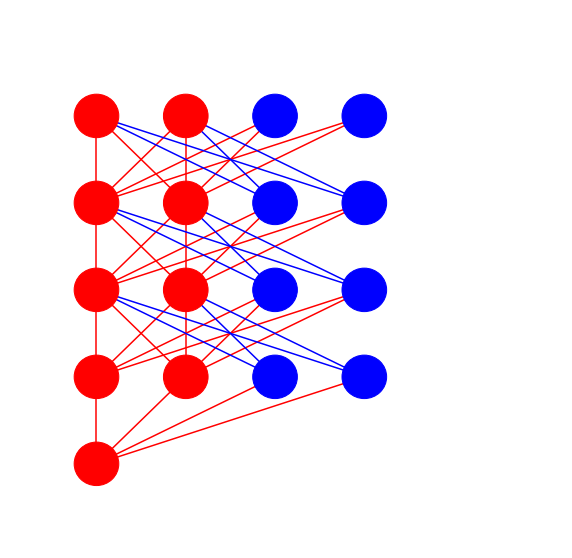
\includegraphics[width=\textwidth]{figures/feedforward network.png}
\end{frame}

\begin{frame}
    \frametitle{Results - 5: feed-forward networks}
    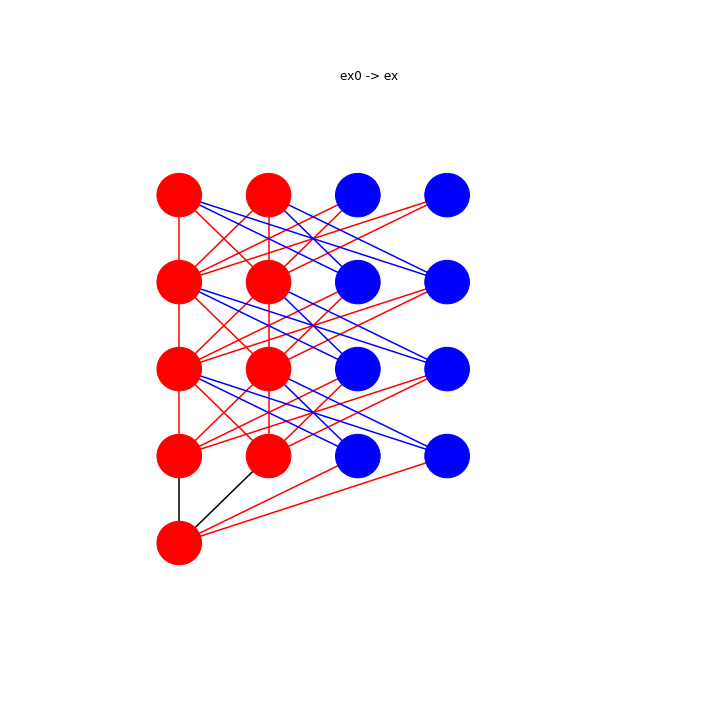
\includegraphics[width=\textwidth]{figures/ex0 -> ex.png}
\end{frame}

\begin{frame}
    \frametitle{Results - 5: feed-forward networks}
    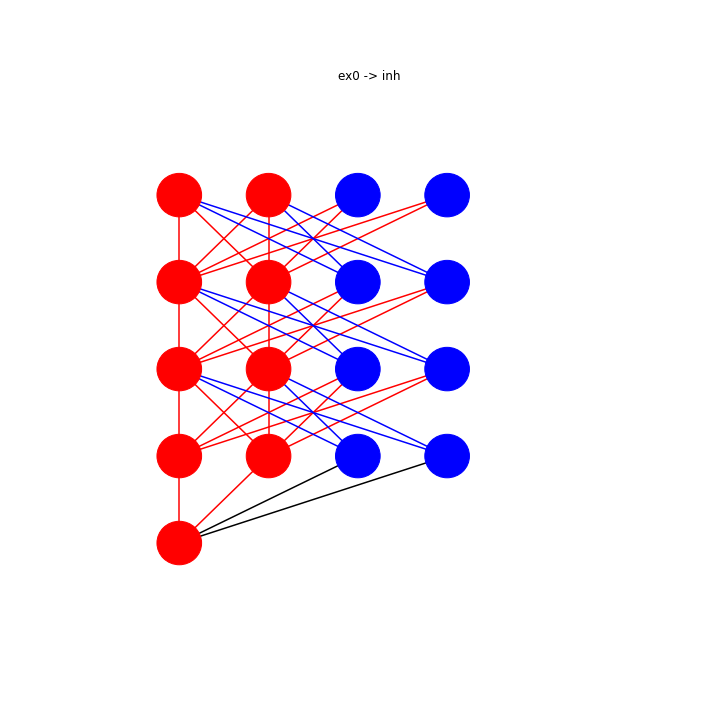
\includegraphics[width=\textwidth]{figures/ex0 -> inh.png}
\end{frame}

\begin{frame}
    \frametitle{Results - 5: feed-forward networks}
    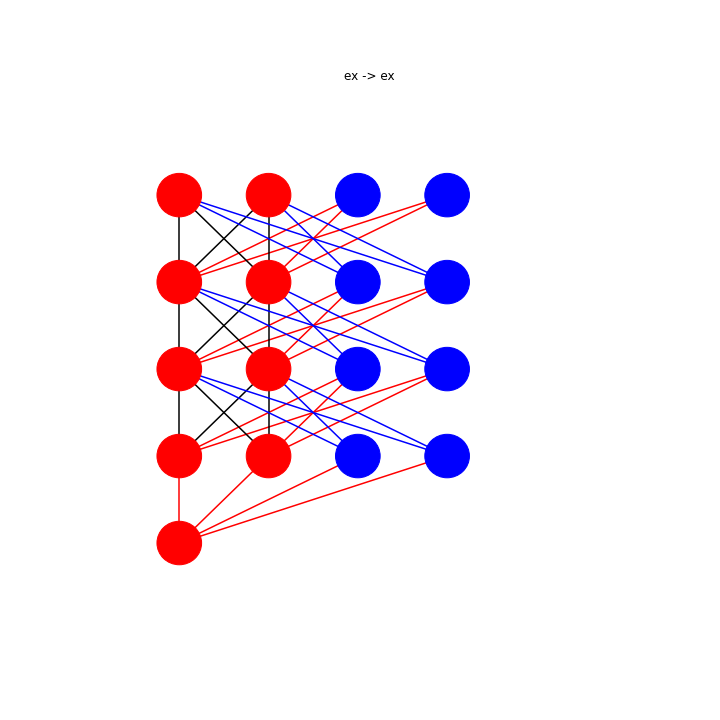
\includegraphics[width=\textwidth]{figures/ex -> ex.png}
\end{frame}

\begin{frame}
    \frametitle{Results - 5: feed-forward networks}
    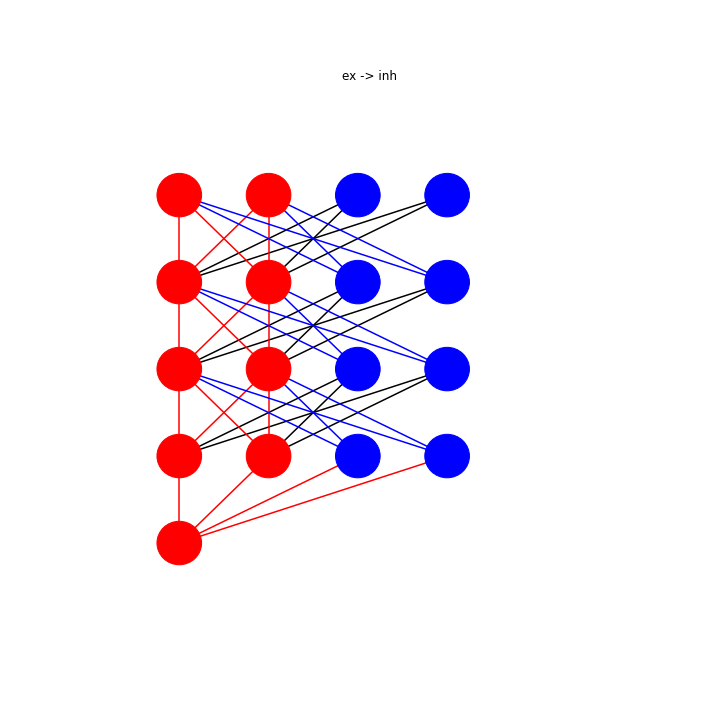
\includegraphics[width=\textwidth]{figures/ex -> inh.png}
\end{frame}

\begin{frame}
    \frametitle{Results - 5: feed-forward networks}
    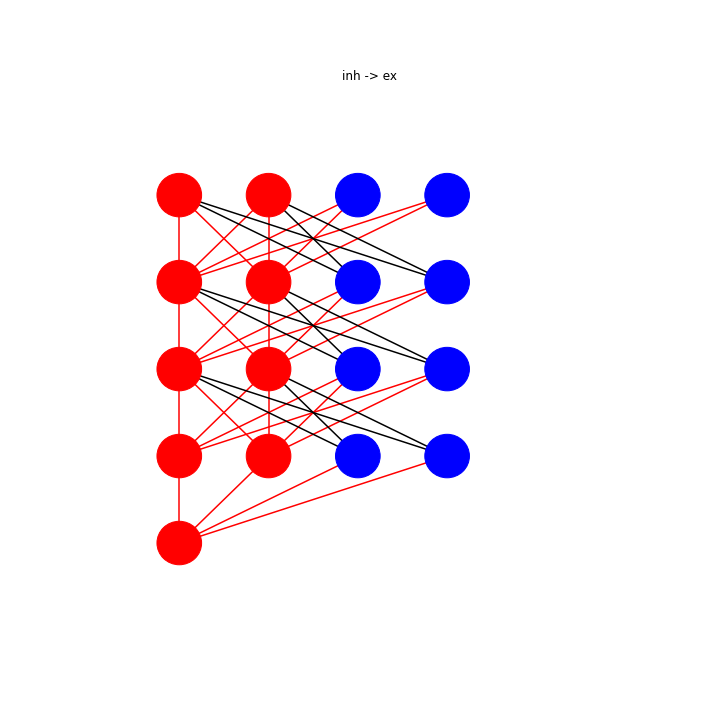
\includegraphics[width=\textwidth]{figures/inh -> ex.png}
\end{frame}

\begin{frame}
    \frametitle{Results - 5: feed-forward networks}
    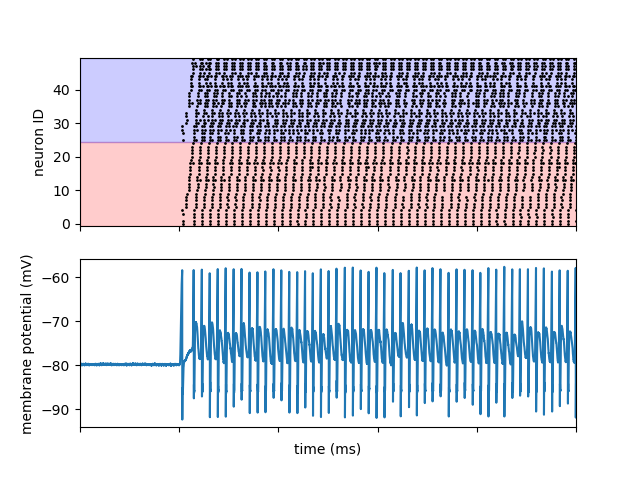
\includegraphics[width=\textwidth]{figures/feedforward signals loop.png}
\end{frame}

\begin{frame}
    %%%M
    \frametitle{Results - 6: recurrent networks}
    %%%
    \begin{columns}
          \column{0.5\linewidth}
          	\begin{figure}
    				\centering
    				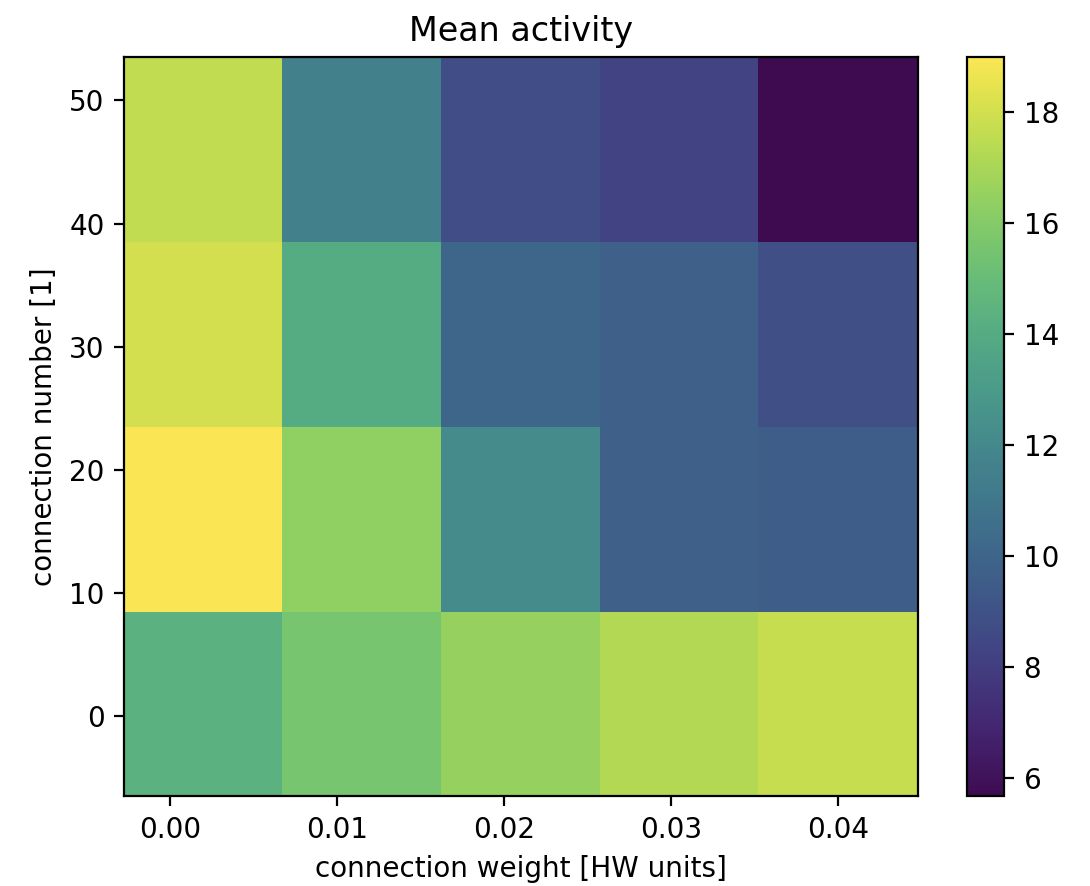
\includegraphics[width=\linewidth]{figures/activity_sweep.png}
    				%\caption{source: FP09 neuromorphic computing script,  2020}
 		   \end{figure}
 		   \begin{itemize}
          		\item Spikey as a collection of LiF circuits interconnected with synapses
          	\end{itemize}

          \column{0.5\linewidth}
          \begin{figure}
    				\centering
    				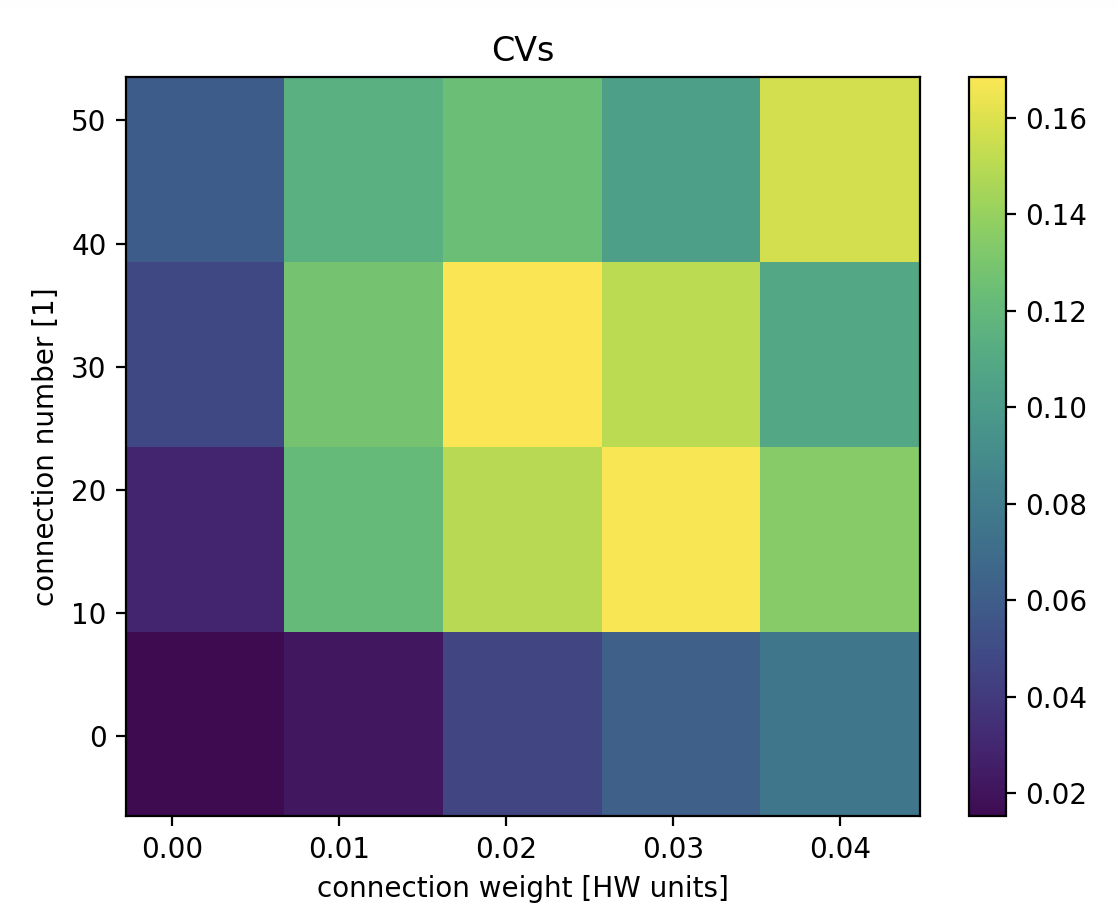
\includegraphics[width=\linewidth]{figures/CV_sweep.png}
    				%\caption{source: FP09 neuromorphic computing script,  2020}
 		   \end{figure}
 		   \begin{itemize}
          		\item Schematic of the basic operation process
          	\end{itemize}

	\end{columns}

\end{frame}

\begin{frame}
    \frametitle{Results - 7: simple computation XOR}
    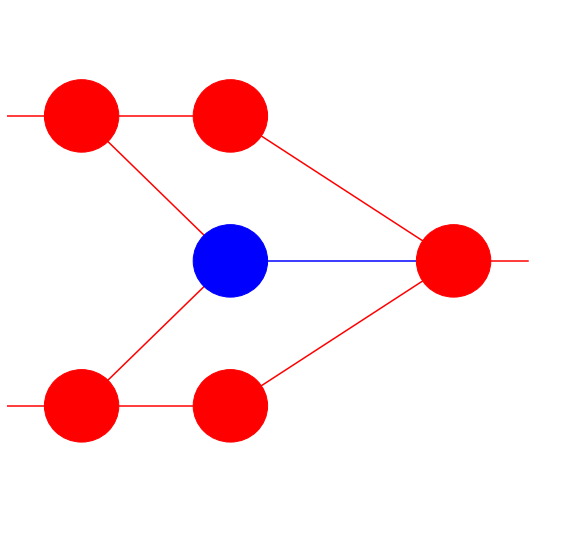
\includegraphics[width=\textwidth]{figures/XOR-suggestion.png}
\end{frame}

\begin{frame}
    \frametitle{Results - 7: simple computation XOR}
    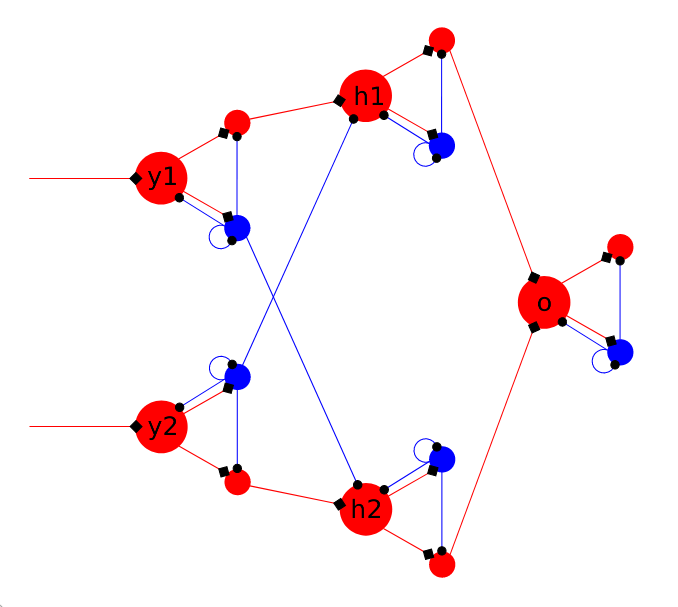
\includegraphics[width=.7\textwidth]{figures/XOR-used.png}
\end{frame}

\begin{frame}
    \frametitle{Results - 7: simple computation XOR}
    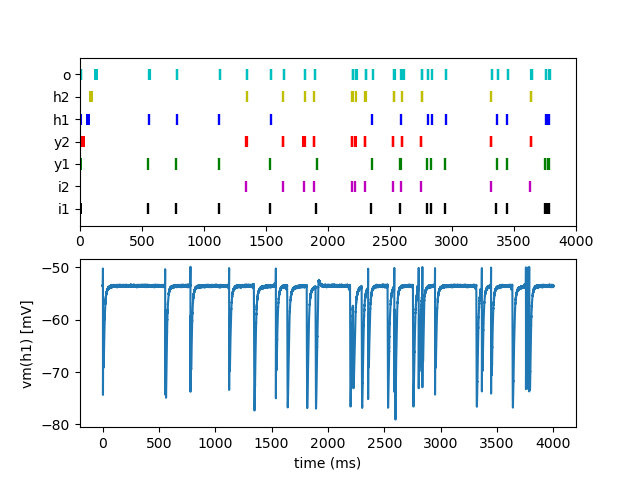
\includegraphics[width=\textwidth]{figures/XOR-output.png}
\end{frame}

\begin{frame}
   \frametitle{Conclusion}
   \begin{itemize}
       \item Possible to run more complex networks
       \item High instability $\rightarrow$ not production worthy
   \end{itemize}
\end{frame}

\begin{frame}
    %%%
    \frametitle{Discussion}
    %%%
    \begin{itemize}
        \item Desirable: measurability of stability
            \begin{itemize}
                \item $\tau(T)$
                \item $T(t)$
            \end{itemize}
        \item Low population sizes in experiment
    \end{itemize}
\end{frame}

\end{document}
